\documentclass[12pt,a4paper]{article}
\usepackage[utf8]{inputenc}
\usepackage[spanish]{babel}
\usepackage{amsmath}
\usepackage{amsfonts}
\usepackage{amssymb}
\usepackage[left=2cm,right=2cm,top=2cm,bottom=2cm]{geometry}
\usepackage{graphicx}
\usepackage{enumerate}
\author{Yoleivys Delgado}
\title{\textbf{Movimiento de Proyectiles}}

\begin{document}
\maketitle
El movimiento de proyectil es una forma de movimiento donde un cuerpo o partícula es lanzado cerca de la superficie terrestre y adquiere un movimiento a lo largo de una trayectoria parabólica bajo la acción de la gravedad. En este tipo de movimiento se considera la resistencia con el aire despreciable. La figura (\ref{fig:figura1})  describe la trayectoria seguida en un movimiento parabólico.

\begin{figure}[htbp]
 \centering
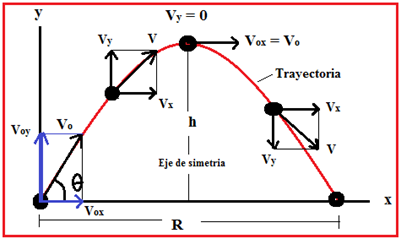
\includegraphics[width=10cm]{figura1.png} 
\caption{Trayectoria seguida por un proyectil} \label{fig:figura1}
\end{figure}

\section{ Velocidad inicial}

La velocidad inicial del cuerpo en un movimiento parabólico es descrito por un vector que tiene componente horizontal y vertical.Este vector puede determinase mediante la siguiente ecuación:
\begin{equation}
v_0 = v_{0x}i+ v_{0y}j 
\end{equation}

Donde las componentes en \textbf{x} y \textbf{y} están dadas por:

\begin{eqnarray}
v_{0x} =v_{0} cos (\theta)\\
v_{0y} =v_{0} sin (\theta)
\end{eqnarray}

\section{Aceleración}

Como solo hay aceleración en la dirección vertical, el movimiento horizontal es rectilineo uniforme, en tanto el  movimiento vertical es del tipo caída libre, entonces las respectivas aceleraciones vienen dadas por:
\begin{eqnarray}
a_{x} =0\\
a_{y} =-g
\end{eqnarray}

\section{Velocidad}
Dado que la aceleración de la partícula en $x$ es cero, se tiene que la componente horizontal de la velocidad permanece constante durante todo la trayectoria, pero la componente vertical disminuye  hasta que alcanza la altura máxima donde es nula. En el retorno del cuerpo a la superficie terrestre la velocidad empieza a aumentar debido a la acción de la gravedad. La figura muestra el vector velocidad en diferentes puntos de la trayectoria.

Sus componentes están dadas por:

\begin{eqnarray}
v_{0x} =v_{0} cos (\theta)\\
v_{0y} =v_{0} sin (\theta)- g t
\end{eqnarray}

\section{Desplazamiento}
A un tiempo $t$ los desplazamientos vertical y horizontal del cuerpo o proyectil están dados por :
\begin{eqnarray}
x = v_{0} t cos (\theta)\\
y = v_{0} t sin (\theta) - \frac{1}{2} g t^2
\end{eqnarray}

\section{Tiempo de vuelo}
El tiempo de vuelo, es el tiempo total que demora el proyectil  en el aire, de la ecuación anterior tenemos que:
\begin{equation}
y = v_{0} t sin (\theta) - \frac{1}{2} g t^2 \nonumber
\end{equation}
Al final del vuelo el proyectil retorna al eje vertical, en este caso $y=0$, entonces tenemos 
\begin{equation}
0 = v_{0} t sin (\theta) - \frac{1}{2} g t^2 \nonumber
\end{equation}
\begin{equation}
v_{0} t sin (\theta) = \frac{1}{2} g t^2\nonumber
\end{equation}
\begin{equation}
v_{0} sin (\theta) = \frac{1}{2} g t \nonumber
\end{equation}
\begin{equation}
t = \frac{2v_{0}sin (\theta)}{g}
\end{equation}

\section{ Altura máxima del proyectil}
Cuando el proyectil alcanza la altura máxima su $v_{y} =0$, de $10$ tenemos que el tiempo para alcanzar la altura máxima es:
\begin{equation}
t_{h_{max}} = \frac{v_{0}sin (\theta)}{g}
\end{equation}

Usando 9 tenemos

\begin{equation}
h=v_{0} t_{h_{max}}sin(\theta)-\frac{1}{2}gt_{h_{max}}^2
\end{equation}
 
Sustituyendo 11 en 12, llegamos a:
\begin{equation}
h=\frac{v_{0}^2 sin(\theta)^2}{2g}   
\end{equation}

\section{ Distancia horizontal máxima del proyectil}
La distancia horizontal del proyectil es la distancia que este viaja, es decir cuando el proyectil retorna a la tierra $(y=0)$

\begin{eqnarray}
d = v_0 t_d cos(\theta)
\end{eqnarray}
donde $t_d$ es el tiempo de vuelo dado por la ecuación 10
así, la distancia horizontal esta dada por 
\begin{equation}
d = \frac{v_0^2}{g}sin(2\theta)
\end{equation}

Se puede notal que d es máximo cuando $ sin(2\theta)= 1$, lo cual corresponde cuando
\begin{eqnarray}
2\theta =90 \nonumber\\
\theta = 45 \nonumber
\end{eqnarray}

\section{Ejemplo}

un cuerpo es lanzado desde la superficie terrestre con una velocidad de $25 m/s $ a un ángulo de $35^{o}$. Determine
\begin{enumerate}[a)]

\item El tiempo de vuelo del proyectil. 
\item La altura máxima 
\item Distancia horizontal maxima alcanzada por el proyectil.
\end{enumerate}

\textbf{solución }\\
\textbf{a)} La ecuación para determinar el tiempo de vuelo es $t = \frac{2v_{0}sin (\theta)}{g}$, donde tendriamos que:\\
\begin{eqnarray}
t = \frac{2 (25\hspace{0.2cm} m/s) sin (35)}{9.8\hspace{0.2cm} m/s^{2}}\nonumber\\ 
t = 2.926\hspace{0.2cm}  segundos \nonumber
\end{eqnarray}

\textbf{b)} La ecuación para determinar la altura máxima alcanzada por el proyectil es:\\ $h_{max}=\frac{v_{0}^2 sin(\theta)^2}{2g} $, donde tendriamos que:\\
\begin{eqnarray}
h_{max}=\frac{(25\hspace{0.2cm} m/s)^2 sin(35)^2}{2(9.8\hspace{0.2cm} m/s^{2})} \nonumber\\ 
h_{max} = 10.49\hspace{0.2cm}  metros\nonumber
\end{eqnarray}

\textbf{c)} La ecuación para determinar la altura distancia horizontal maxima alcanzada por el proyectil es:\\ $d_{max} = \frac{v_0^2}{g}sin(2\theta) $, donde tendriamos que:\\
\begin{eqnarray}
d_{max} = \frac{(25\hspace{0.2cm} m/s)^2}{9.8\hspace{0.2cm} m/s^{2}}sin(2(35))\nonumber\\ 
d_{max} = 60.0 \hspace{0.2cm} metros\nonumber
\end{eqnarray}
En el apendice siguiente encontrata el codigo Fortran utilizado pra los incisos a al c
\newpage
\section{Apéndice}
\subsection{Tiempo de vuelo}
\begin{verbatim}
program tiempo_vuelo

  implicit none

  ! definimos constantes
  real, parameter :: g = 9.8
  real, parameter :: pi = 3.1415927

  ! definimos las variables
  real :: a, v0, tv

 
  write(*,*) 'Dame el ángulo y la rapidez inicial'
  read(*,*) a, v0

  ! convirtiendo ángulo a radianes
  a = a * pi / 180.0

  ! la ecuacion de tiempo de vuelo es
  tv = (2 * v0 * sin (a))/ g

  !escribiendo el resultado en la pantalla
  write(*,*) 'tiempo de vuelo es = ', tv, ' segundos'

  end program tiempo_vuelo
\end{verbatim}
\newpage
\subsection{Altura máxima}
\begin{verbatim}
program altura_maxima

  implicit none

  ! definimos constantes
  real, parameter :: g = 9.8
  real, parameter :: pi = 3.1415927

  ! definimos las variables
  real :: a, v0, hm


  write(*,*) 'Dame el ángulo y la rapidez inicial'
  read(*,*) a, v0

  ! convirtiendo ángulo a radianes
  a = a * pi / 180.0
  ! la ecuacion de tiempo de vuelo es
  hm = (v0**2  * (sin (a))**2)/( 2 * g)
  

  !escribiendo el resultado en la pantalla
  write(*,*) 'la altura maxima es  = ', hm, ' metros'

 
  end program altura_maxima

\end{verbatim}
\newpage
\subsection{Distancia horizontal máxima} 
\begin{verbatim}
program distancia_maxima

  implicit none

  ! definimos constantes
  real, parameter :: g = 9.8
  real, parameter :: pi = 3.1415927

  ! definimos las variables
  real :: a, v0, xm

  write(*,*) 'Dame el ángulo y la rapidez inicial'
  read(*,*) a, v0

  ! convirtiendo ángulo a radianes
  a = a * pi / 180.0
  ! la ecuacion de tiempo de vuelo es
  xm = (v0**2  * (sin (2 * a)))/ g
  

  !escribiendo el resultado en la pantalla
  write(*,*) 'la distancia  maxima es  = ', xm, ' metros'

 
  end program distancia_maxima
\end{verbatim}
\subsection*{tttt}
\end{document}